\begingroup
\definecolor{GraphSpectrumNode}{HTML}{E5EAF0}
\definecolor{GraphSpectrumOutline}{HTML}{7188A3}
\definecolor{GraphSpectrumEdge}{HTML}{4C4D4F}
\definecolor{GraphSpectrumText}{HTML}{3B4252}
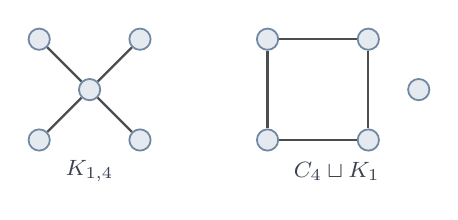
\begin{tikzpicture}[x=8mm,y=8mm,
  vertex/.style={circle,inner sep=0pt,minimum size=2.7mm,
    fill=GraphSpectrumNode,draw=GraphSpectrumOutline,line width=.65pt},
  every path/.style={line width=.8pt},
  title/.style={text=GraphSpectrumText,font=\footnotesize}]
  \begin{scope}
    \node[vertex] (s) at (0,0) {};
    \node[vertex] (l1) at (-.8,.8) {};
    \node[vertex] (l2) at (.8,.8) {};
    \node[vertex] (l3) at (.8,-.8) {};
    \node[vertex] (l4) at (-.8,-.8) {};
    \foreach \v in {l1,l2,l3,l4} {
      \draw[GraphSpectrumEdge] (s) -- (\v);
    }
    \node[title] at (0,-1.3) {$K_{1,4}$};
  \end{scope}
  \begin{scope}[xshift=29mm]
    \node[vertex] (c1) at (-.8,.8) {};
    \node[vertex] (c2) at (.8,.8) {};
    \node[vertex] (c3) at (.8,-.8) {};
    \node[vertex] (c4) at (-.8,-.8) {};
    \node[vertex] at (1.6,0) {};
    \draw[GraphSpectrumEdge] (c1) -- (c2) -- (c3) -- (c4) -- (c1);
    \node[title] at (.3,-1.3) {$C_4\sqcup K_1$};
  \end{scope}
\end{tikzpicture}
\endgroup
